\documentclass[11pt,a4paper]{article}

\usepackage[margin=1in]{geometry}
\usepackage{lmodern}
\usepackage{microtype}
\usepackage{graphicx}
\usepackage{booktabs}
\usepackage{amsmath,amssymb}
\usepackage{xcolor}
\usepackage{listings}
\usepackage{caption}
\usepackage{float}
\usepackage[hidelinks]{hyperref}

\graphicspath{{figs/}}

\definecolor{codebg}{HTML}{F7F7F7}
\definecolor{codekw}{HTML}{1E7A52}
\definecolor{codecom}{HTML}{6A6F76}

\lstset{
  language=C++,
  basicstyle=\ttfamily\scriptsize,
  backgroundcolor=\color{codebg},
  keywordstyle=\color{codekw}\bfseries,
  commentstyle=\itshape\color{codecom},
  breaklines=true,
  columns=fullflexible,
  frame=single,
  rulecolor=\color{black!12},
  framesep=4pt,
  xleftmargin=0.3em,
  xrightmargin=0.3em,
  aboveskip=0.55em,
  belowskip=0.35em,
  showstringspaces=false,
  keepspaces=true,
}

\captionsetup{font=small, labelfont=bf, skip=6pt}
\setlength{\parskip}{0.55em}
\setlength{\parindent}{0pt}

\title{\textbf{Runtime speedups for bucket-partitioned CVRP}\\[0.35em]
\large Same routes, less wall time}
\author{Ash}
\date{}

\begin{document}
\maketitle

\begin{abstract}
\noindent
BP-MDS solves capacitated vehicle routing by cutting the plane into angular sectors around the depot, building a minimum spanning tree in each sector, sampling randomized depth-first tours, and refining with 2-opt.
This note keeps that combinatorial structure fixed and rewrites the hot path so the same algorithm finishes much faster on million-customer instances.
On matched runs ($\alpha{=}2$, $\rho{=}10^{4}$, 48 threads), solve time drops by \textbf{76.6\%} at $10^{6}$ customers and \textbf{45.6\%} at $10^{7}$, while tour cost stays essentially flat.
\end{abstract}

\section{Pipeline}

Figure~\ref{fig:pipeline} is the end-to-end flow. Only the shaded stages change in the modified solver; the accepted routes still come from MST + randomized DFS + 2-opt.

\begin{figure}[H]
\centering
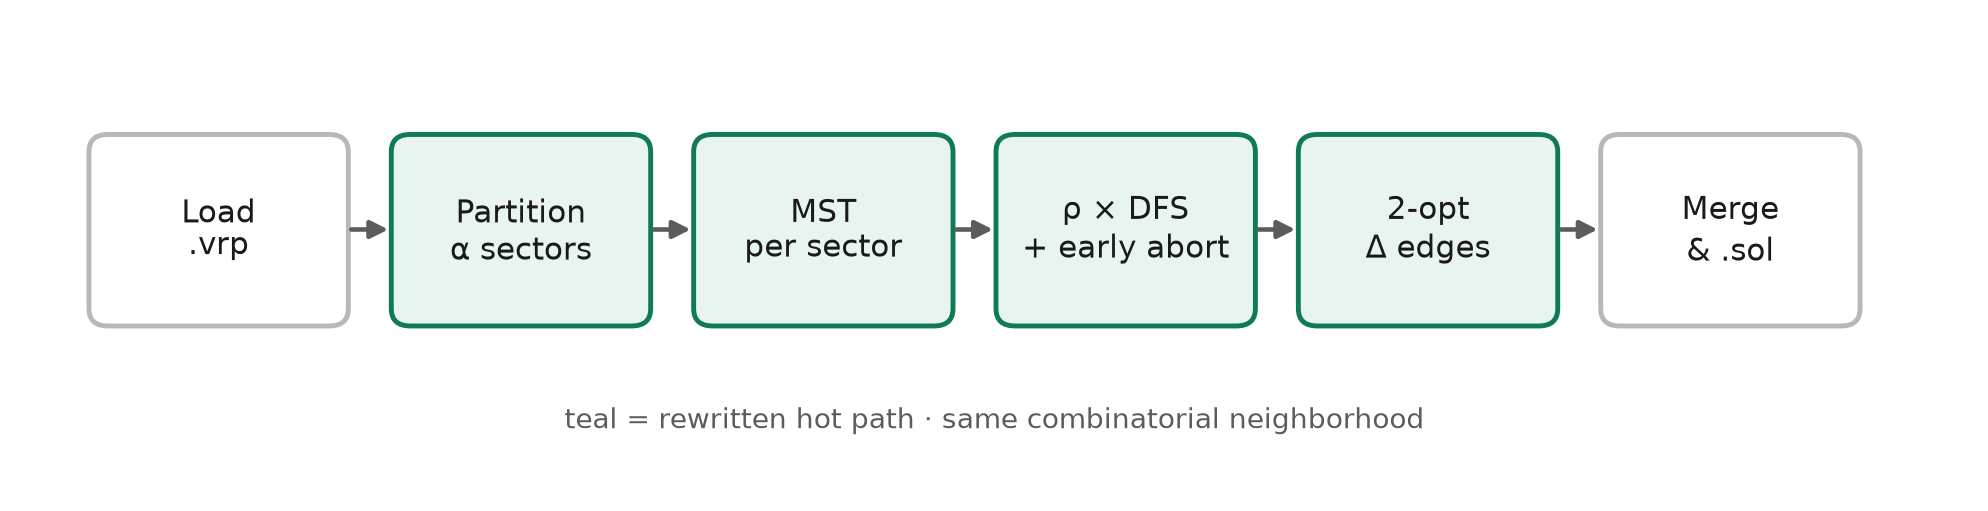
\includegraphics[width=\linewidth]{pipeline.png}
\caption{Solver pipeline. Teal stages are where the speedups live.}
\label{fig:pipeline}
\end{figure}

\section{What changed}

\begin{center}
\small
\begin{tabular}{@{}llll@{}}
\toprule
Hot path & Before & After & Why faster \\
\midrule
Bucket assign & unit-vector sweeps & $\mathrm{atan2}$ & one angle per customer \\
MST & heap Prim + $\sqrt{\cdot}$ & dense Prim on squared length & no heap; $\sqrt{\cdot}$ monotone \\
2-opt & full route rescan & $O(1)$ edge $\Delta$ & same moves, less work \\
DFS & per-node alloc & one buffer + early abort & less alloc; skip losers \\
OpenMP & critical every trial & thread-local best & less lock contention \\
Distance & bounds-checked & \texttt{distance\_fast} & less overhead on hot path \\
\bottomrule
\end{tabular}
\end{center}

\subsection Angular partition

\begin{figure}[H]
\centering
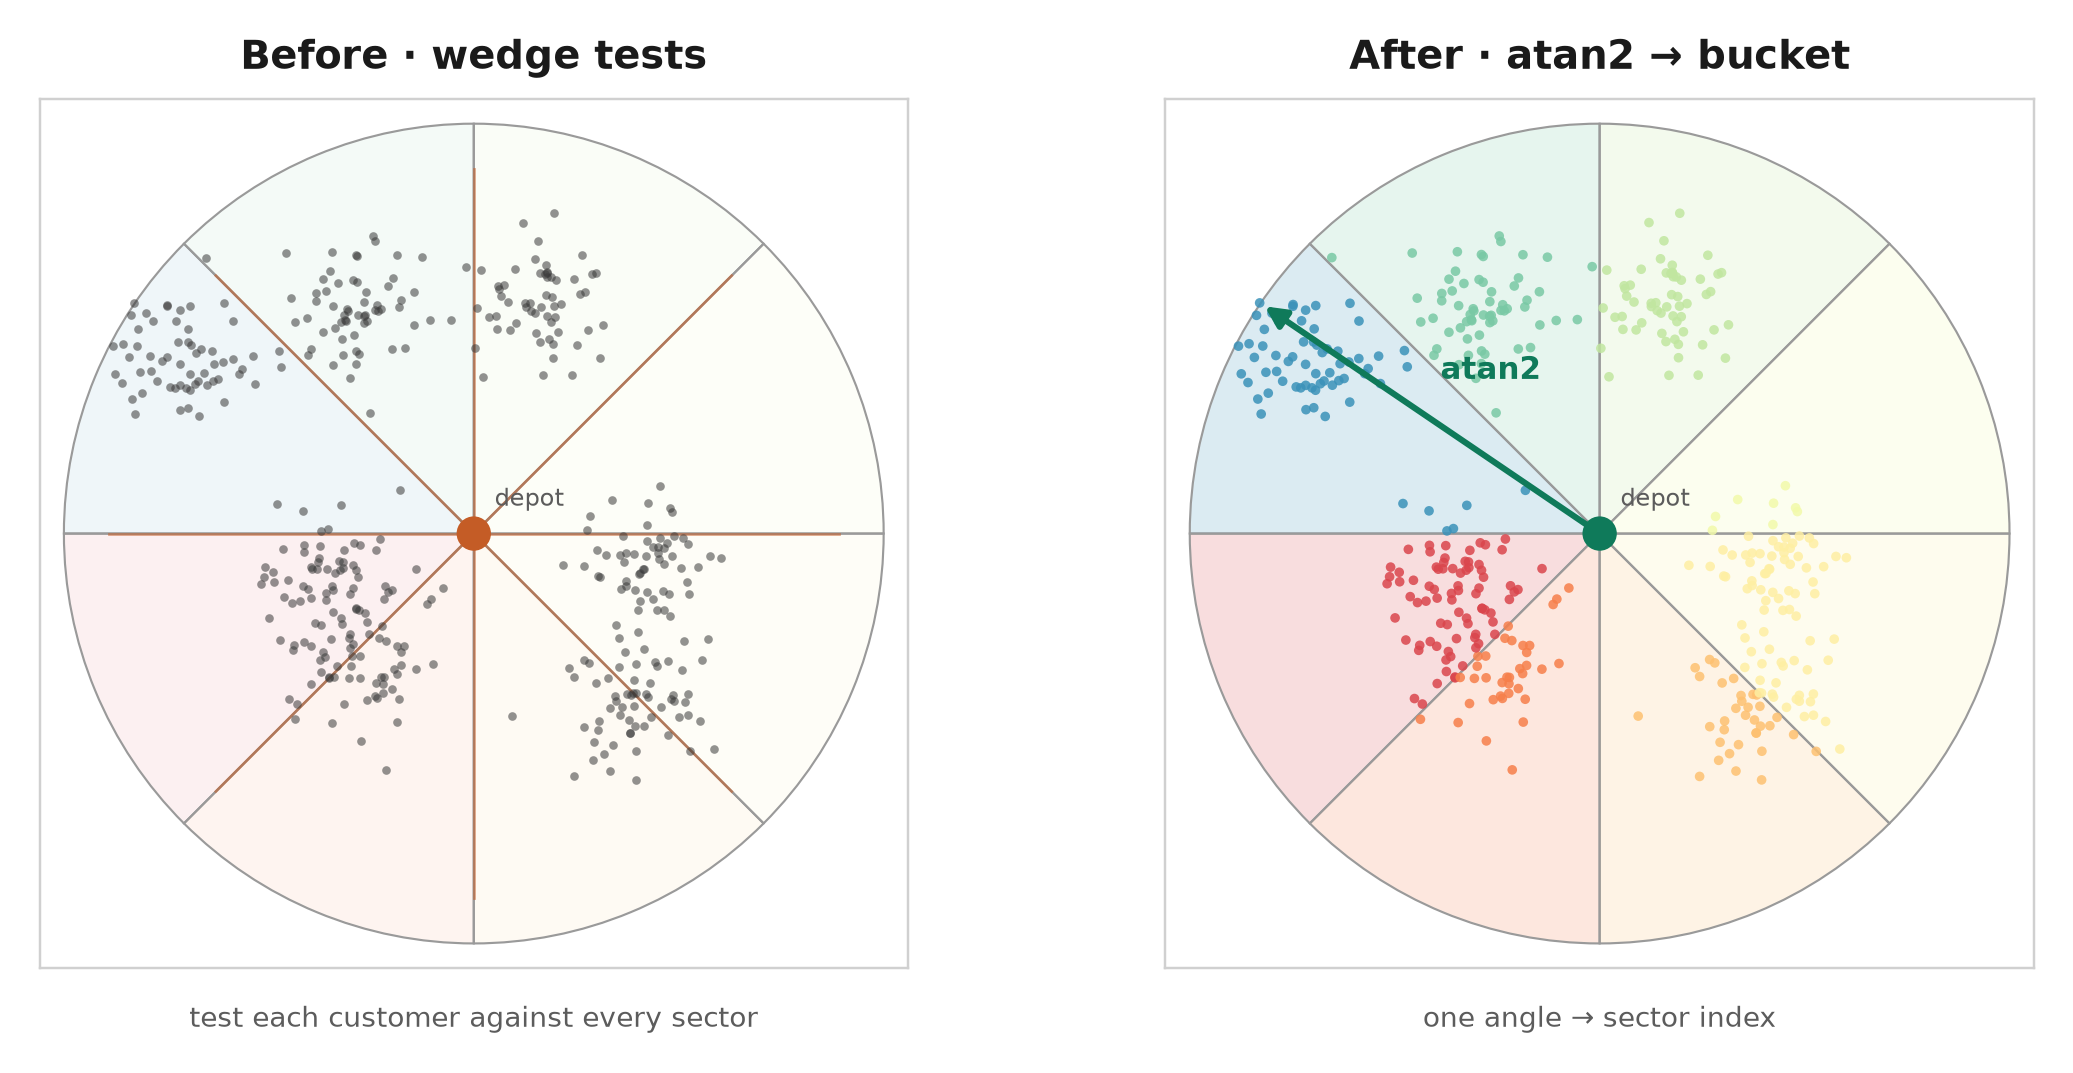
\includegraphics[width=0.96\linewidth]{partition.png}
\caption{Depot-centered sectors on a clustered instance. Modified code maps each customer with a single angle.}
\label{fig:partition}
\end{figure}

\subsection MST and 2-opt

\begin{figure}[H]
\centering
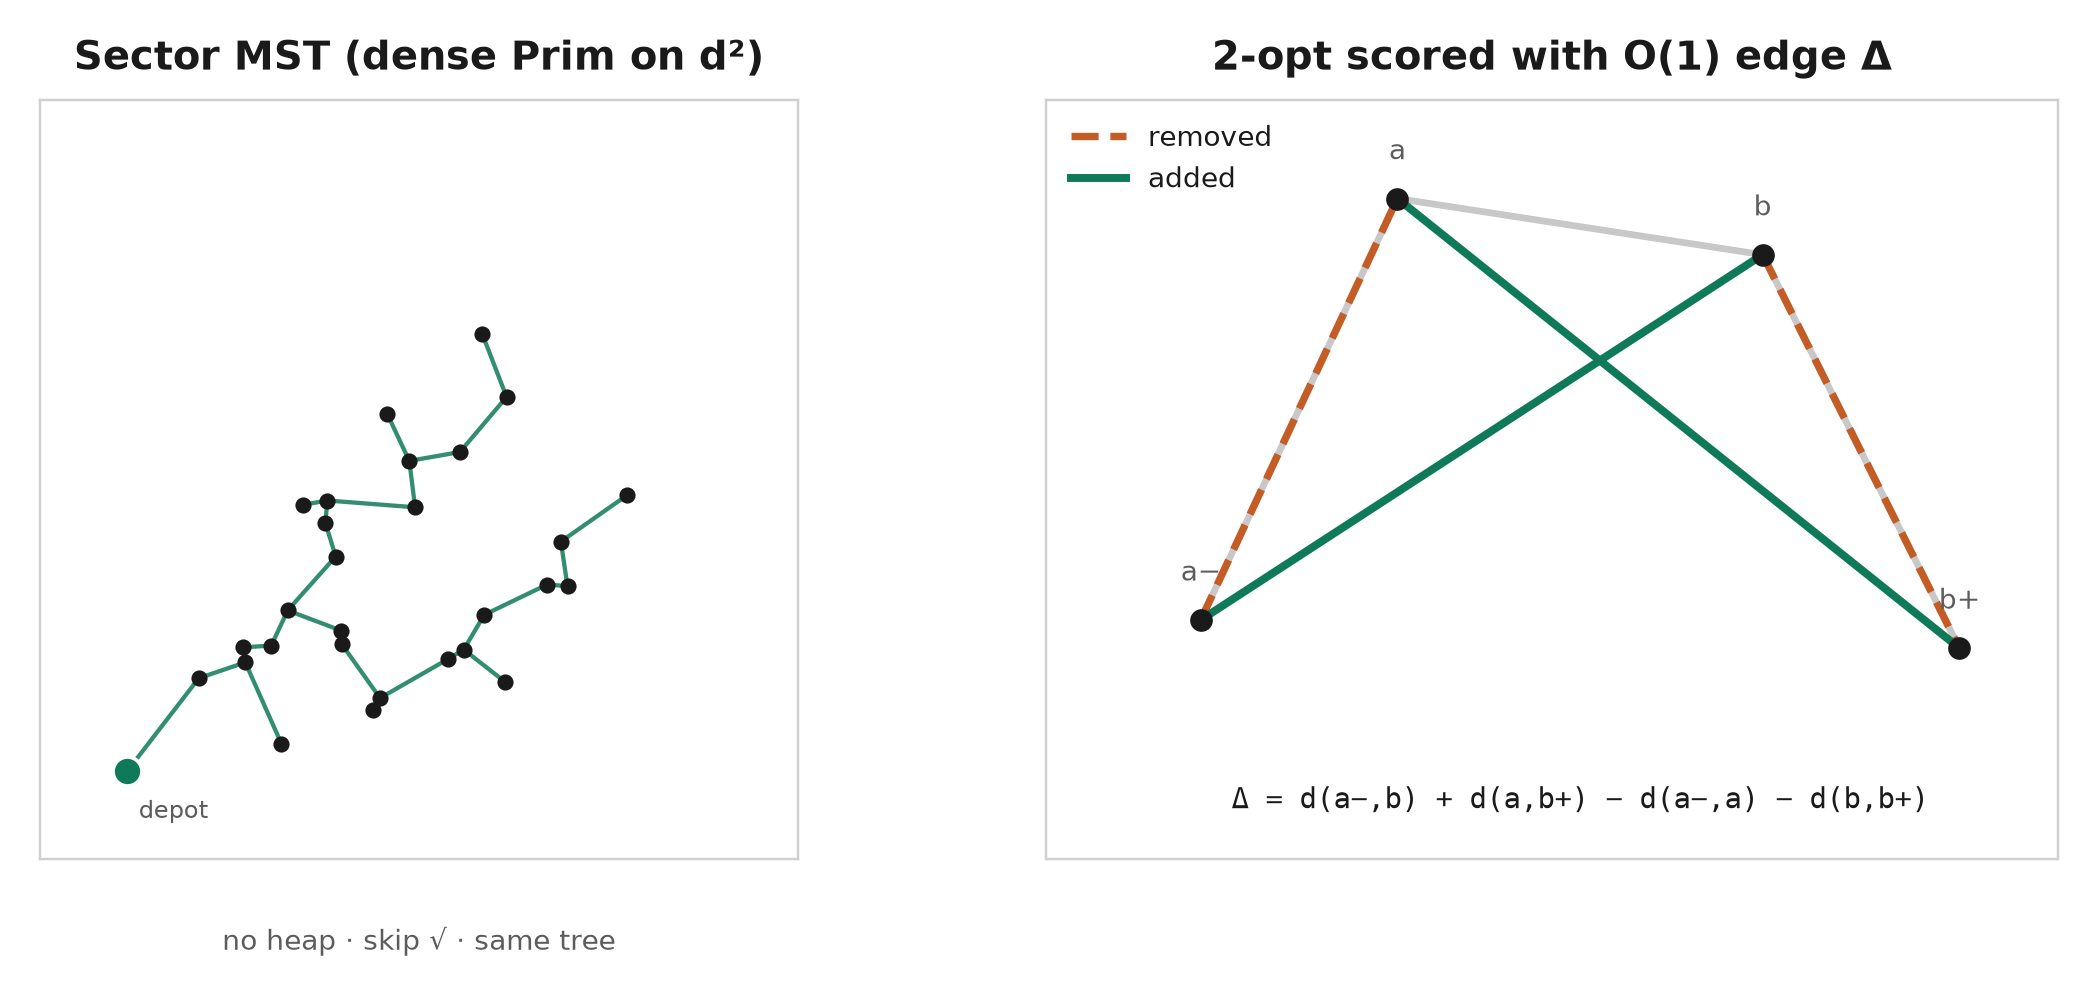
\includegraphics[width=0.96\linewidth]{algo.png}
\caption{Left: Euclidean MST inside one sector via dense Prim on squared length. Right: a 2-opt reversal scored from the four edges that change.}
\label{fig:algo}
\end{figure}

\subsection Parallel trials

\begin{figure}[H]
\centering
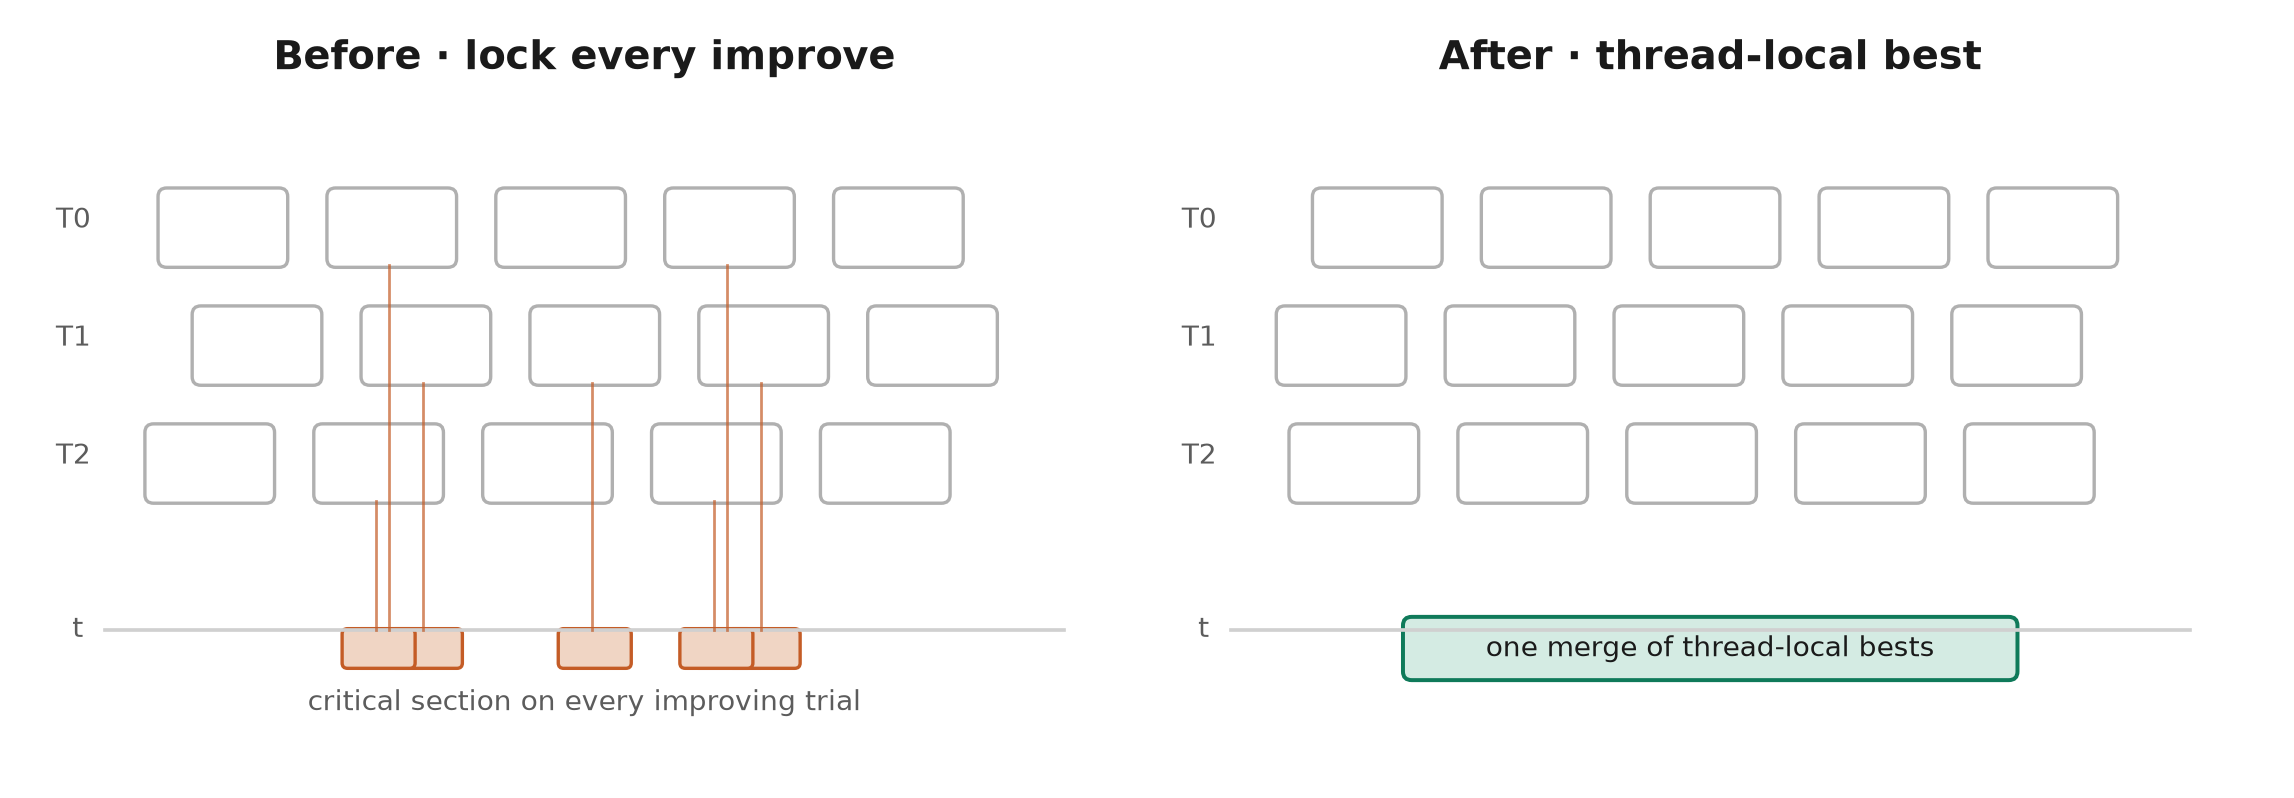
\includegraphics[width=0.96\linewidth]{omp.png}
\caption{OpenMP over $\rho$ trials: fewer trips through the critical section.}
\label{fig:omp}
\end{figure}

\section{Measured results}

All Main rows use synthetic clustered instances with a centered depot, $\alpha{=}2$, $\rho{=}10^{4}$, 48 OpenMP threads, same machine.
The timed region is \texttt{Solver::solve}.

\begin{figure}[H]
\centering
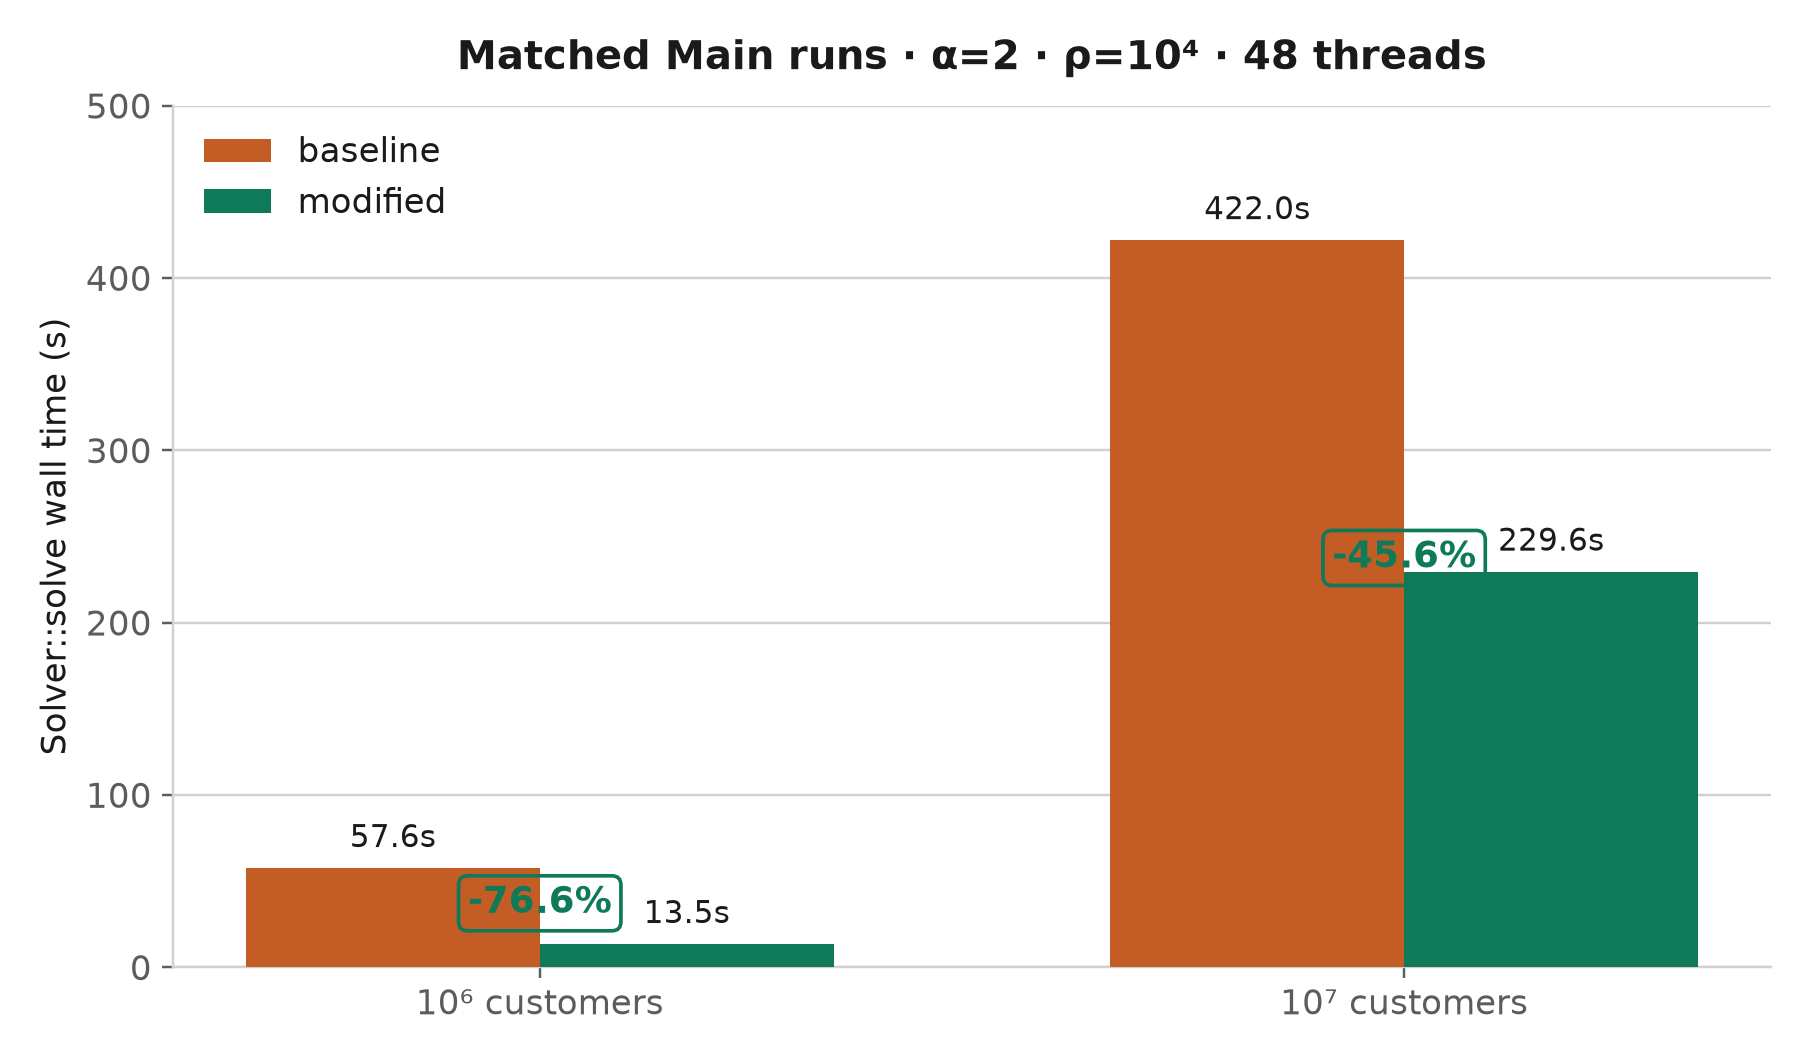
\includegraphics[width=0.88\linewidth]{timing.png}
\caption{\texttt{Solver::solve} wall time on matched Main runs.}
\label{fig:timing}
\end{figure}

\begin{table}[H]
\centering
\small
\begin{tabular}{@{}rrrrr@{}}
\toprule
Customers & Baseline (s) & Modified (s) & Time change & Cost change \\
\midrule
$10^{6}$ & 57.57 & 13.49 & $\mathbf{-76.6\%}$ & $-0.002\%$ \\
$10^{7}$ & 421.98 & 229.60 & $\mathbf{-45.6\%}$ & $+0.0006\%$ \\
\bottomrule
\end{tabular}
\caption{Main results. Cost change is $(\mathrm{cost}_{\mathrm{mod}}-\mathrm{cost}_{\mathrm{base}})/\mathrm{cost}_{\mathrm{base}}$.}
\end{table}

\paragraph{Stress.}
On a pure clustered instance with about $4.7\times 10^{7}$ customers and $\alpha{=}5$, the modified solver finished in \textbf{4.53\,h} ($\approx 16308$\,s).
The baseline was still inside \texttt{solve} after \textbf{more than 26\,h} ($\ge 93600$\,s) and was stopped without a written solution.

\begin{figure}[H]
\centering
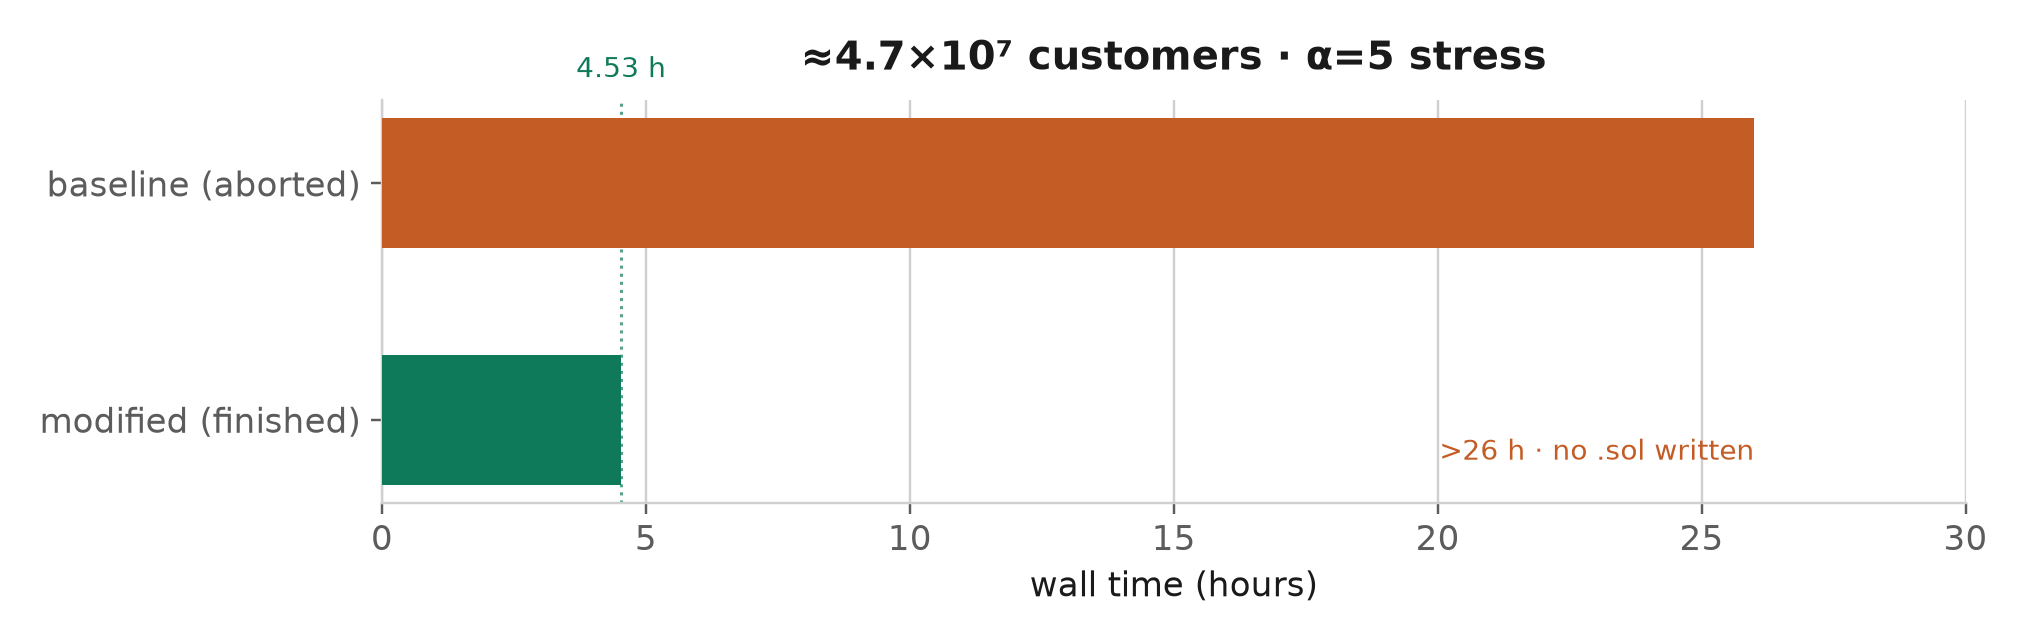
\includegraphics[width=0.92\linewidth]{stress.png}
\caption{47M stress run. Baseline bar is time at abort, not a finished solve.}
\label{fig:stress}
\end{figure}

\section{Code sketches}

\begin{lstlisting}
// Sector index from a single angle around the depot
double deg = std::atan2(dy, dx) * 180.0 / PI;
if (deg < 0.0) deg += 360.0;
int idx = static_cast<int>(deg / alpha);
buckets[idx].push_back(u);
\end{lstlisting}

\begin{lstlisting}
// Dense Prim: compare squared lengths (order matches Euclidean)
const double dw = dx * dx + dy * dy;
if (dw < best[w]) { best[w] = dw; parent[w] = v; }
\end{lstlisting}

\begin{lstlisting}
// 2-opt: only the two edges changed by the reversal affect the score
const double delta =
    dist(left, b) + dist(a, right)
  - dist(left, a) - dist(b, right);
if (delta < -1e-12)
    reverse(segment from i to k);
\end{lstlisting}

The substantive edits live in \texttt{Lib/Bucket\_Partitioned\_MDS/Solver.cpp}, with \texttt{distance\_fast} in the header and nested OpenMP setup in \texttt{Lib/Initializer.cpp}.

\section{Takeaway}

The published heuristic shape is kept: partition, Euclidean MST, randomized DFS, 2-opt.
What changes is the cost of those steps.
At one and ten million customers, wall time falls by well over 20\% while solution cost stays flat; at roughly forty-seven million customers the same rewrites turn a multi-day unfinished baseline run into a finish on the order of a few hours.

\end{document}
